\begin{frame}[fragile]{Visualização de um grafo esparso ponderado não direcionado}

    \begin{figure}
        \centering

        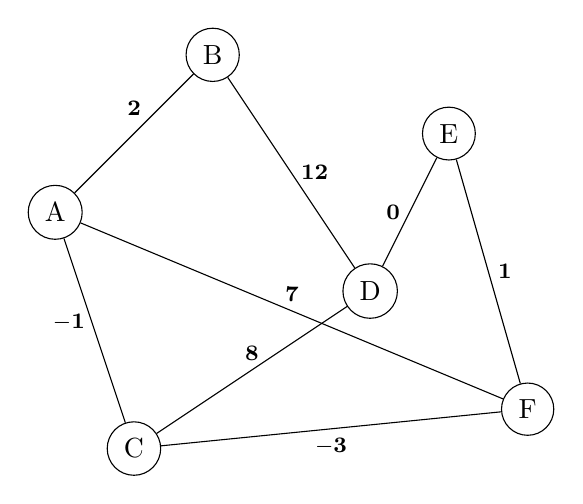
\begin{tikzpicture}
            \node[draw,circle] (A) at (0, 3) { A };
            \node[draw,circle] (B) at (2, 5) { B };
            \node[draw,circle] (C) at (1, 0) { C };
            \node[draw,circle] (D) at (4, 2) { D };
            \node[draw,circle] (E) at (5, 4) { E };
            \node[draw,circle] (F) at (6, 0.5) { F };

            \draw (A) -- node[anchor=south,yshift=0.1cm] { \footnotesize $\mathbf{2}$ } (B);
            \draw (A) -- node[anchor=east,yshift=0.1cm] { \footnotesize $\mathbf{-1}$ } (C);
            \draw (A) -- node[anchor=south,yshift=0.0cm] { \footnotesize $\mathbf{7}$ } (F);
            \draw (B) -- node[anchor=west,xshift=0.0cm] { \footnotesize $\mathbf{12}$ } (D);
            \draw (D) -- node[anchor=east,yshift=0.0cm] { \footnotesize $\mathbf{0}$ } (E);
            \draw (C) -- node[anchor=south,yshift=0.0cm] { \footnotesize $\mathbf{8}$ } (D);
            \draw (C) -- node[anchor=north,yshift=0.0cm] { \footnotesize $\mathbf{-3}$ } (F);
            \draw (E) -- node[anchor=west,yshift=0.0cm] { \footnotesize $\mathbf{1}$ } (F);
        \end{tikzpicture}

    \end{figure}

\end{frame}
